%% USPSC-Introducao.tex

% ----------------------------------------------------------
% Introdução (exemplo de capítulo sem numeração, mas presente no Sumário)
% ----------------------------------------------------------
\chapter[Introdução]{Introdução}
\label{Introdução}

\section{Contextualização e Motivação}\label{sec-context}

Nos últimos anos, houve um aumento dramático na quantidade de dados criados e compartilhados através da internet. Grande parte desse conteúdo está disponível publicamente e sem custo, representando um suprimento virtualmente ilimitado de dados de treinamento para várias tarefas de modelagem estatística e rotulagem. Essa \q{enxurrada de dados} apresenta desafios significativos, mas também oportunidades revolucionárias para o desenvolvimento de sistemas baseados em dados \cite{SeltzerZ09}.

O crescente volume de dados gerados a partir dessas diversas fontes tem impulsionado uma popularização da inteligência artificial (IA), sobretudo com o uso de aprendizado de máquina, que, de forma sucinta, trata da criação de algoritmos que respondam e se adaptem automaticamente aos dados sem a necessidade de intervenção humana de forma contínua \cite{chiavegatto2015}. Aliado a ferramentas poderosas para o processamento massivo e paralelo de dados, esses avanços têm permitido tanto à indústria quanto à comunidade científica desenvolver modelos altamente eficazes e realizar análises mais sofisticadas. A adoção generalizada de técnicas de aprendizado de máquina tem se mostrado fundamental para desvendar o potencial dos dados disponíveis, resultando em descobertas inovadoras e aplicações transformadoras em diversas áreas, incluindo o setor de saúde \cite{mlaplicadosaude}.

O número de estudos médicos de IA cresceu de forma exponencial no período de 2005 a 2019 \cite{ShortGuide2020}, revelando o forte interesse da comunidade científica em buscar métodos cada vez mais eficazes para aprimorar o cuidado e a qualidade de vida dos pacientes. A aplicação de modelos preditivos de aprendizado de máquina possui um potencial significativo para auxiliar na tomada de decisões em diversas etapas do cuidado à saúde, principalmente no diagnóstico, intervenção e acompanhamento de problemas de saúde \cite{obermeyer2017}.

Na área da saúde, as decisões tomadas pelos sistemas de IA podem ter um impacto significativo na vida das pessoas. Se os usuários não conseguem compreender o processo de tomada de decisão, podem não confiar no sistema, chegando até a rejeitá-lo. Portanto, a capacidade de fornecer uma explicação sobre como e por que uma decisão específica foi feita tornou-se uma qualidade essencial em sistemas desse tipo \cite{WagnerBenedikt2021Ahpo}. Além disso, a explicabilidade também pode auxiliar os desenvolvedores na identificação e correção de erros ou viés nos sistemas de IA, tornando-os mais justos e precisos.

Diante desse contexto, este trabalho se propõe a avaliar diversos modelos de classificação com o objetivo de prever a reinternação hospitalar de pacientes, utilizando um conjunto de dados de cuidados de saúde mental coletados pelo sistema de informação da Coordenação de Internações em Ribeirão Preto, Brasil, de julho de 2012 a dezembro de 2017. A relevância deste tipo de trabalho se dá, pois, por meio dessas previsões, medidas preventivas podem ser adotadas antecipadamente, evitando a necessidade de reinternação e, consequentemente, reduzindo os custos hospitalares, visto que o custo médio das internações é significativamente maior que o custo médio dos atendimentos ambulatoriais \cite{cesconetto2008}. Além da predição, o estudo também utilizará técnicas de inteligência artificial explicável (do inglês: \textit{explainable artificial inteligence} - XAI) a fim de identificar quais variáveis estão mais associadas a casos de reinternação, fornecendo informações relevantes para o desenvolvimento de políticas e medidas preventivas mais eficazes.

A \autoref{img:fluxogeral} apresenta um fluxo geral deste trabalho:

\begin{figure}[H]
	\centering
	\caption{\label{img:fluxogeral}Fluxo geral do trabalho}
	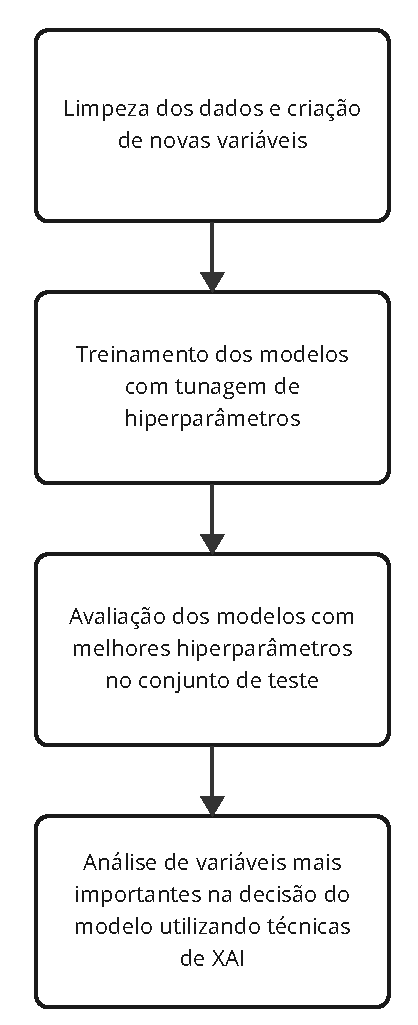
\includegraphics[scale=0.7]{USPSC-img/fluxo-geral-trabalho.pdf}
	\begin{center}
		Fonte: Autor (2023)
	\end{center}
\end{figure}